\section{Решение}

<описание двух моделей>
\\\\
Использован ПК для вычисления: операционная система Ubuntu 18.04 LTS, процессор Intel Pentium 4415U 2.30 ГГц с 4 логическими процессорами
(4 = 1*2*2 --- 1 физический процессор, 2 ядра в физическом процессоре, 2 потока в каждом ядре).


\subsection{Модель 1}

\begin{figure}[H]
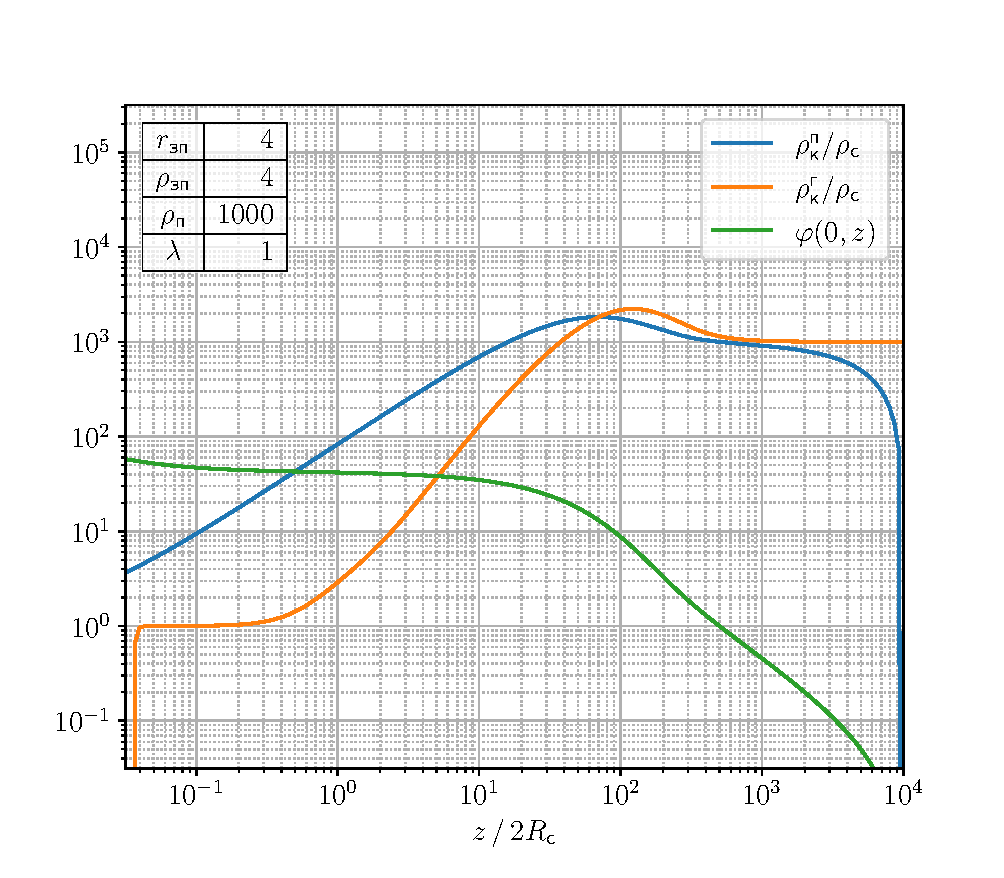
\includegraphics{plot_1_curves}
\caption{}
\label{fig:plot_1_curves}
\end{figure}

Время вычисления решения (рис. \ref{fig:plot_1_curves}) $1.24 \text{ c } \pm 38.3 \text{ мс}$, 7 проходов
($\text{среднее значение} \pm \text{среднеквадратичное отклонение}$ от 7 проходов, в каждом проходе 1 цикл).

6409 узлов расчетной сетки.

Далее изображены поле, расчетная сетка и решение для палетки с этой расчетной сеткой.

\begin{figure}[H]
\centering
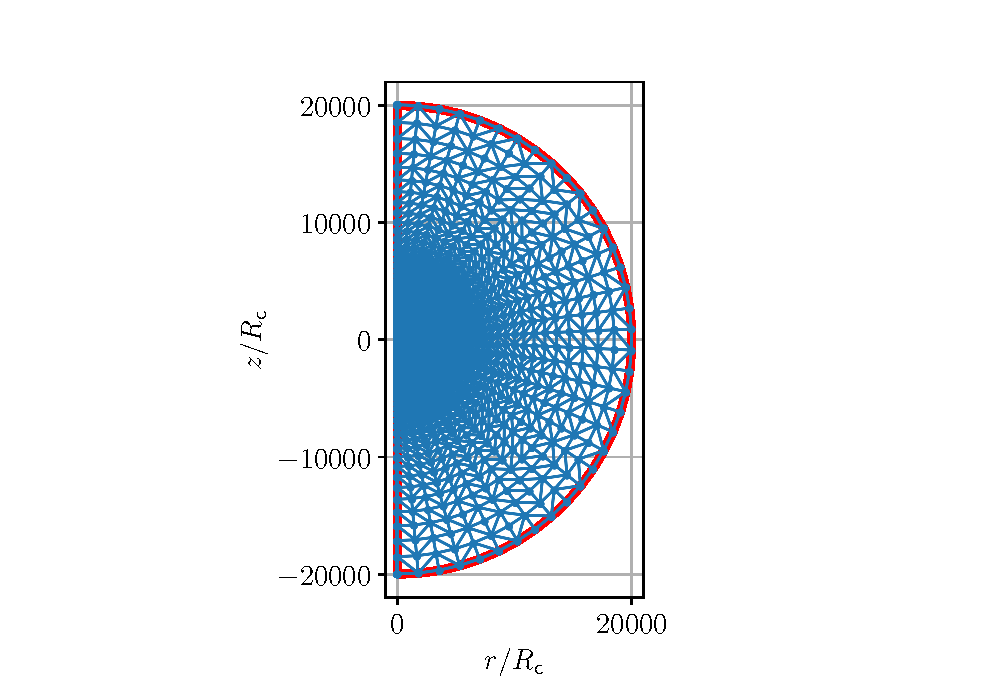
\includegraphics{plot_1_tg_1}
\caption{}
%\label{fig:plot}
\end{figure}

\begin{figure}[H]
\centering
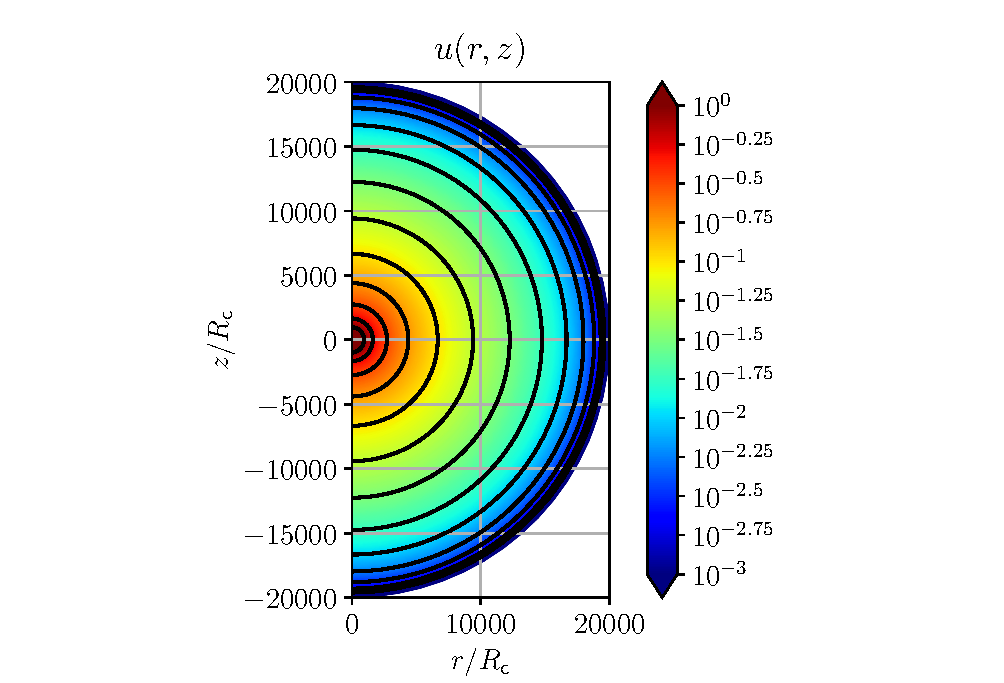
\includegraphics{plot_1_field_1}
\caption{}
%\label{fig:plot}
\end{figure}

\begin{figure}[H]
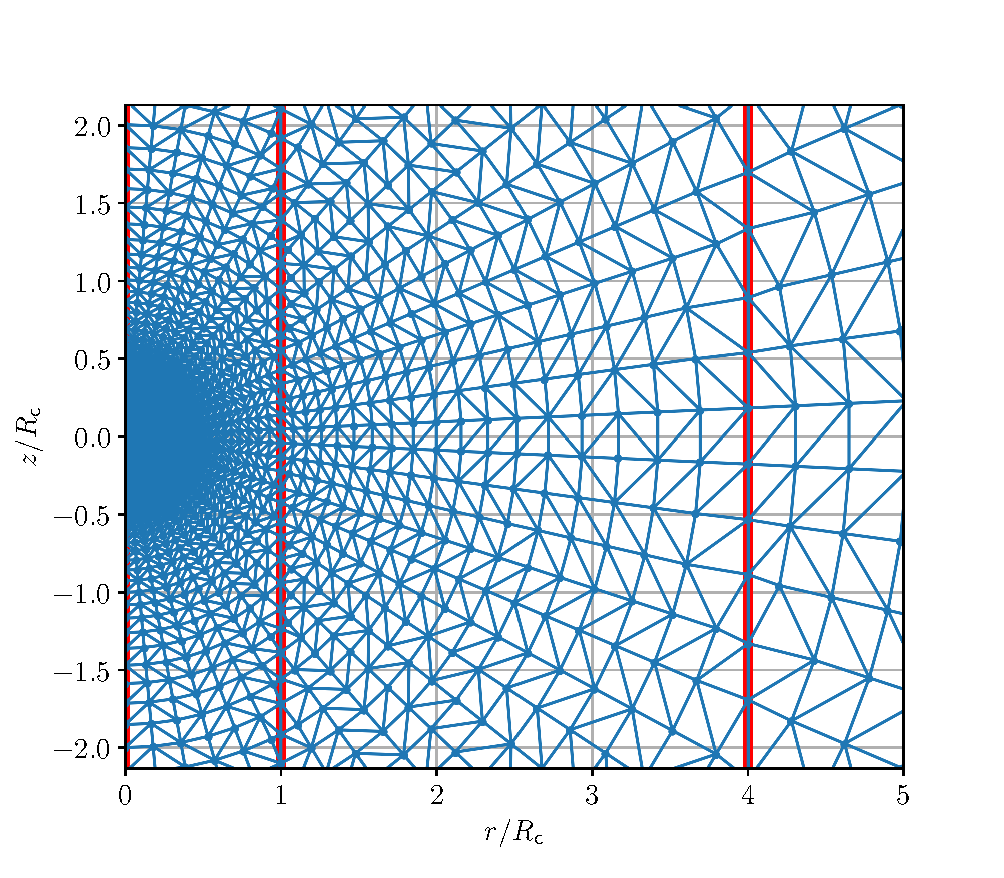
\includegraphics{plot_1_tg_2}
\caption{}
%\label{fig:plot}
\end{figure}

\begin{figure}[H]
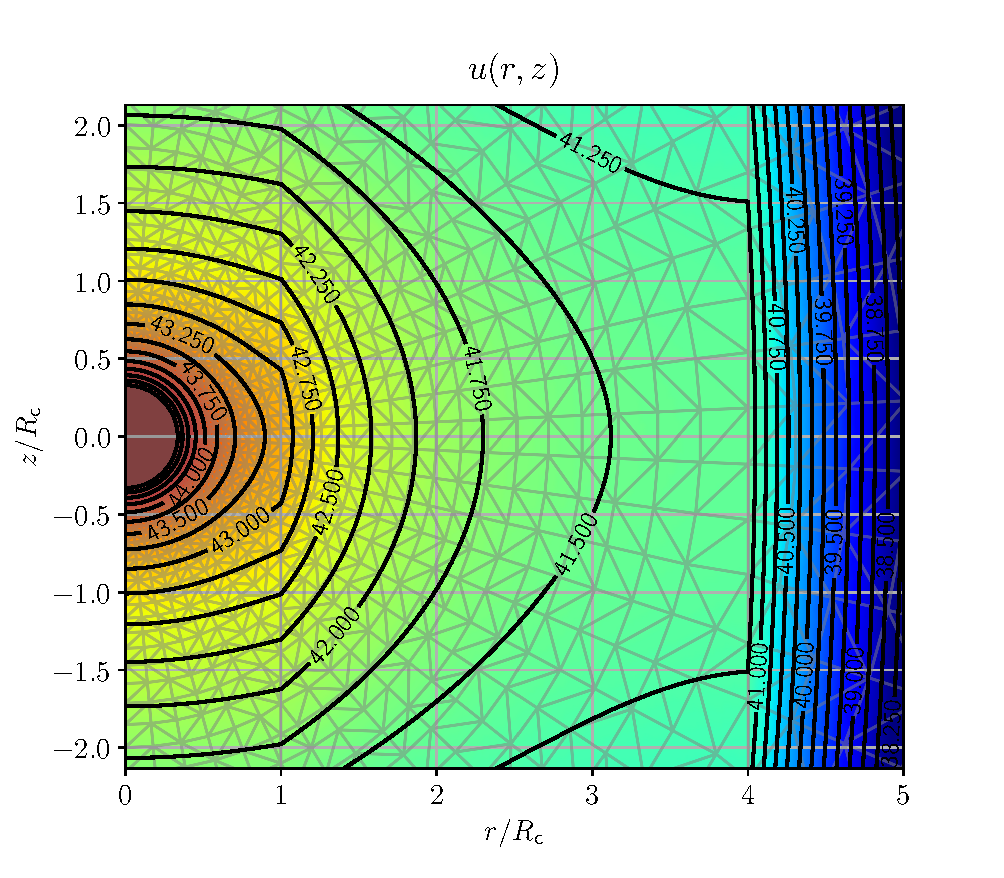
\includegraphics{plot_1_field_2}
\caption{}
%\label{fig:plot}
\end{figure}

\begin{figure}[H]
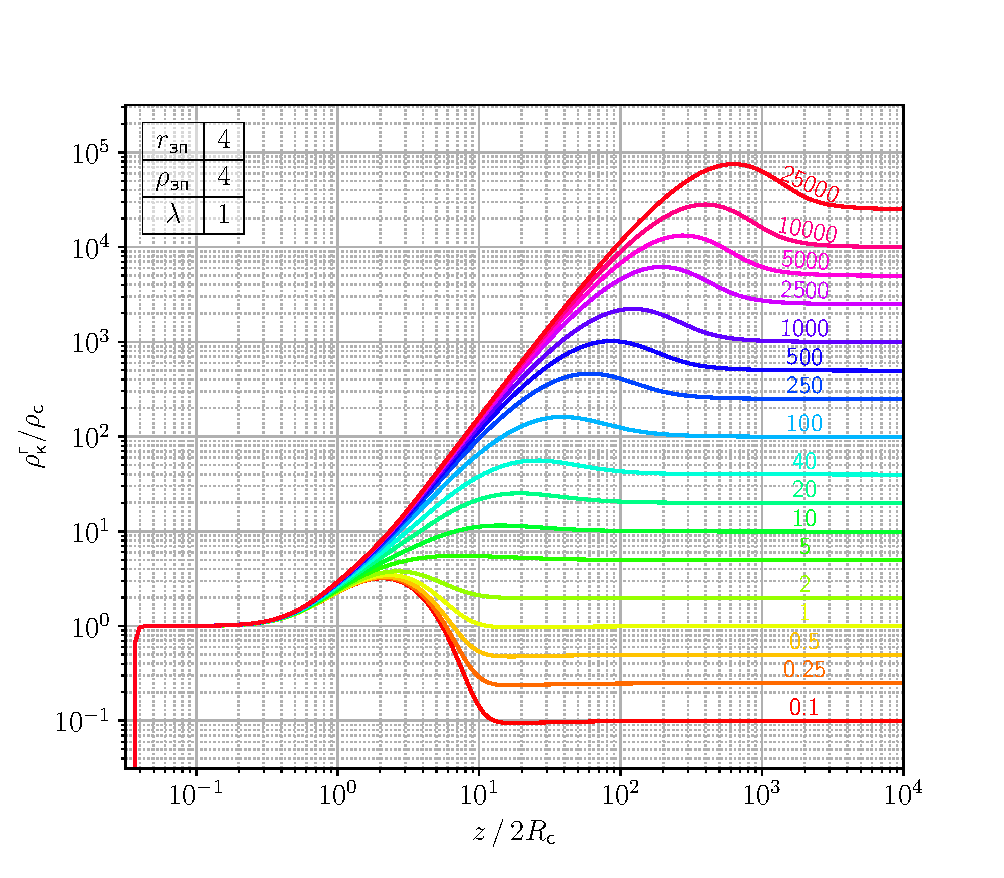
\includegraphics{plot_1_palette}
\caption{}
\end{figure}

Время вычисления палетки $18 \text{ c } \pm 159 \text{ мс}$, 7 проходов.


\newpage
\subsection{Модель 2}

\begin{figure}[H]
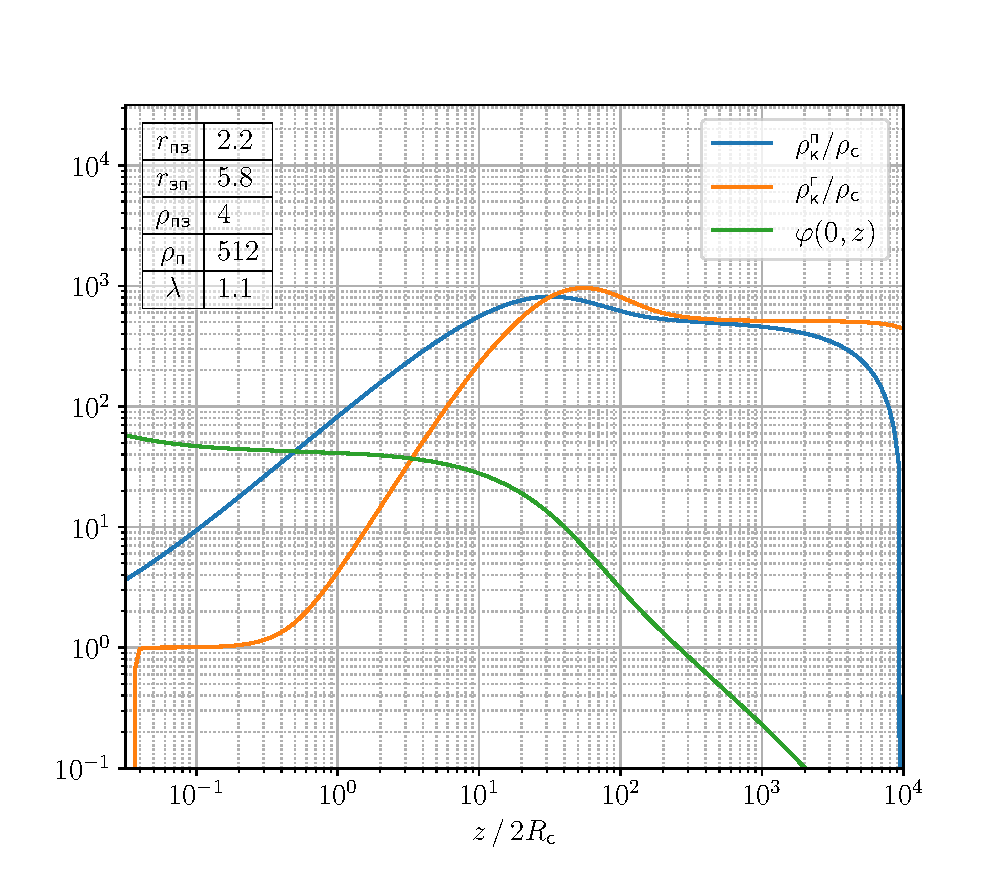
\includegraphics{plot_2_curves}
\caption{}
%\label{fig:plot}
\end{figure}

Время вычисления решения $1.23 \text{ c } \pm 16.3 \text{ мс}$, 7 проходов.

6613 узлов расчетной сетки.

Далее изображены поле, расчетная сетка и решение для палетки с этой расчетной сеткой.

\begin{figure}[H]
\centering
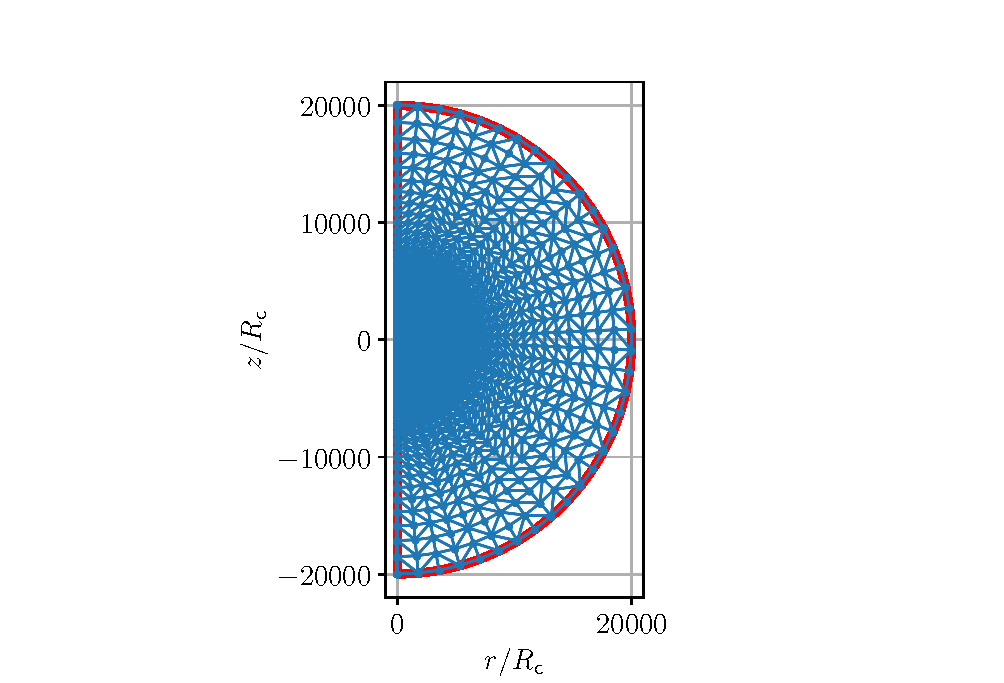
\includegraphics{plot_2_tg_1}
\caption{}
%\label{fig:plot}
\end{figure}

\begin{figure}[H]
\centering
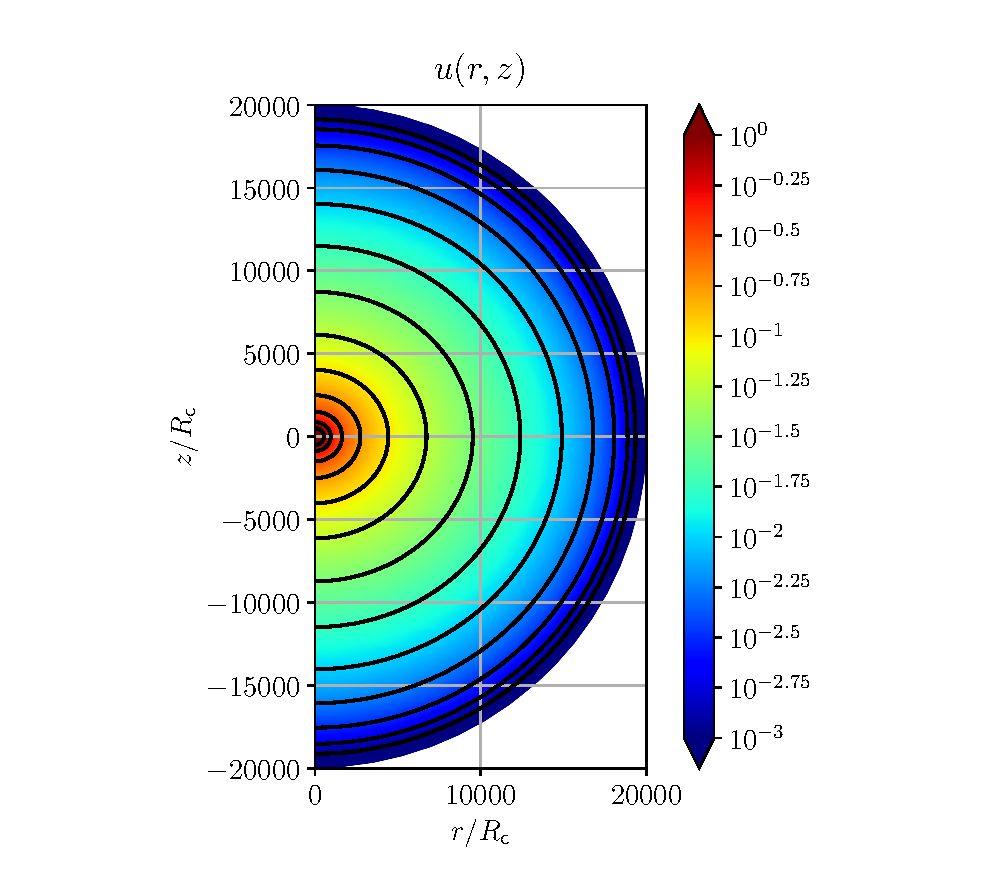
\includegraphics{plot_2_field_1}
\caption{}
%\label{fig:plot}
\end{figure}

\begin{figure}[H]
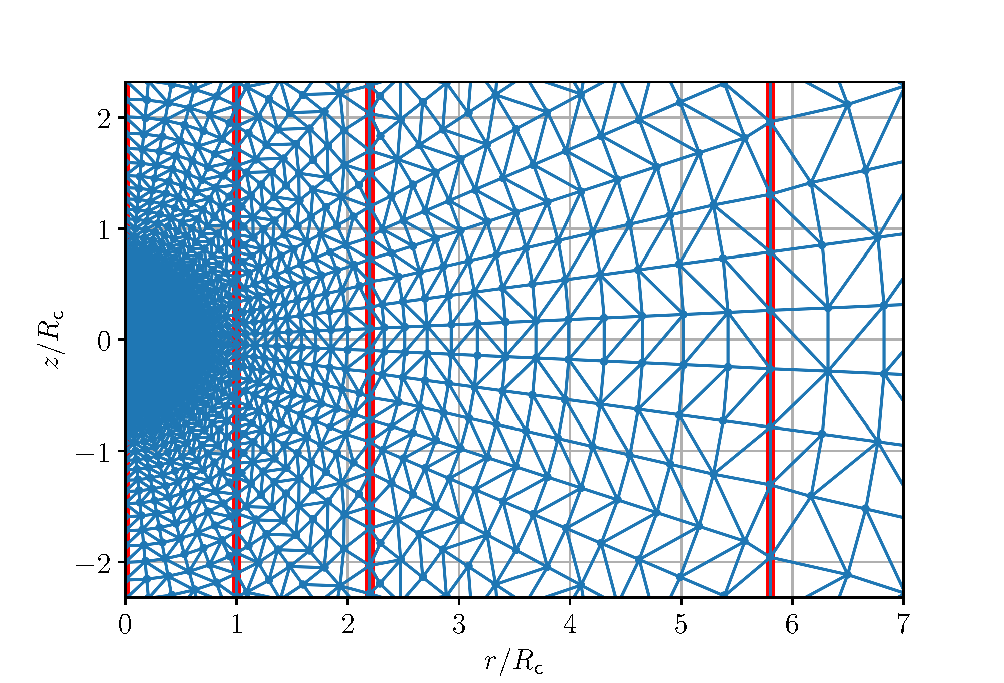
\includegraphics{plot_2_tg_2}
\caption{}
%\label{fig:plot}
\end{figure}

\begin{figure}[H]
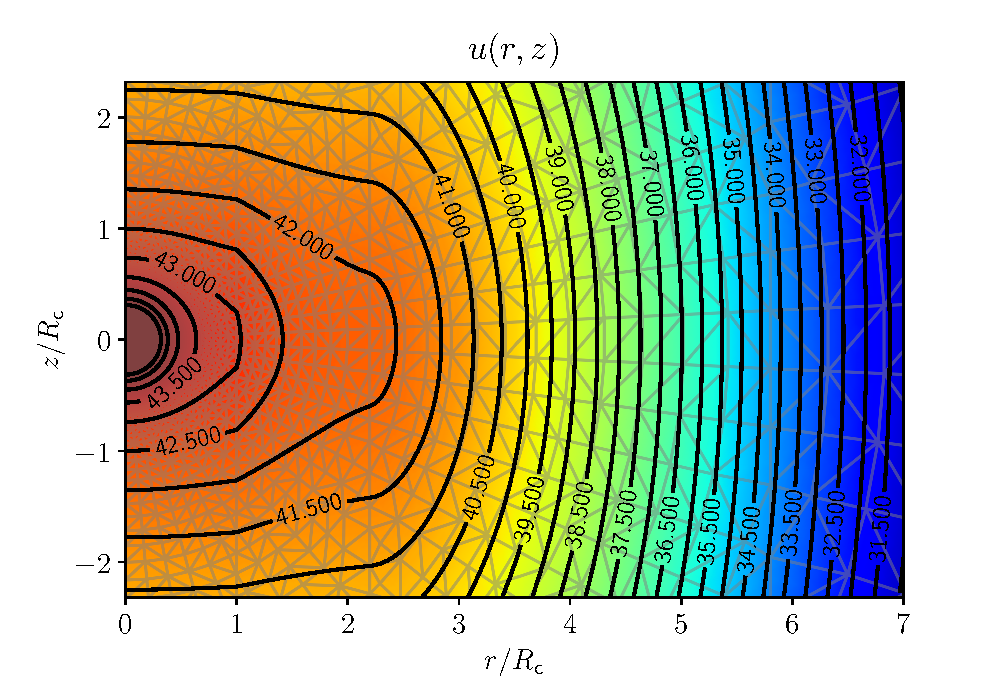
\includegraphics{plot_2_field_2}
\caption{}
%\label{fig:plot}
\end{figure}

\begin{figure}[H]
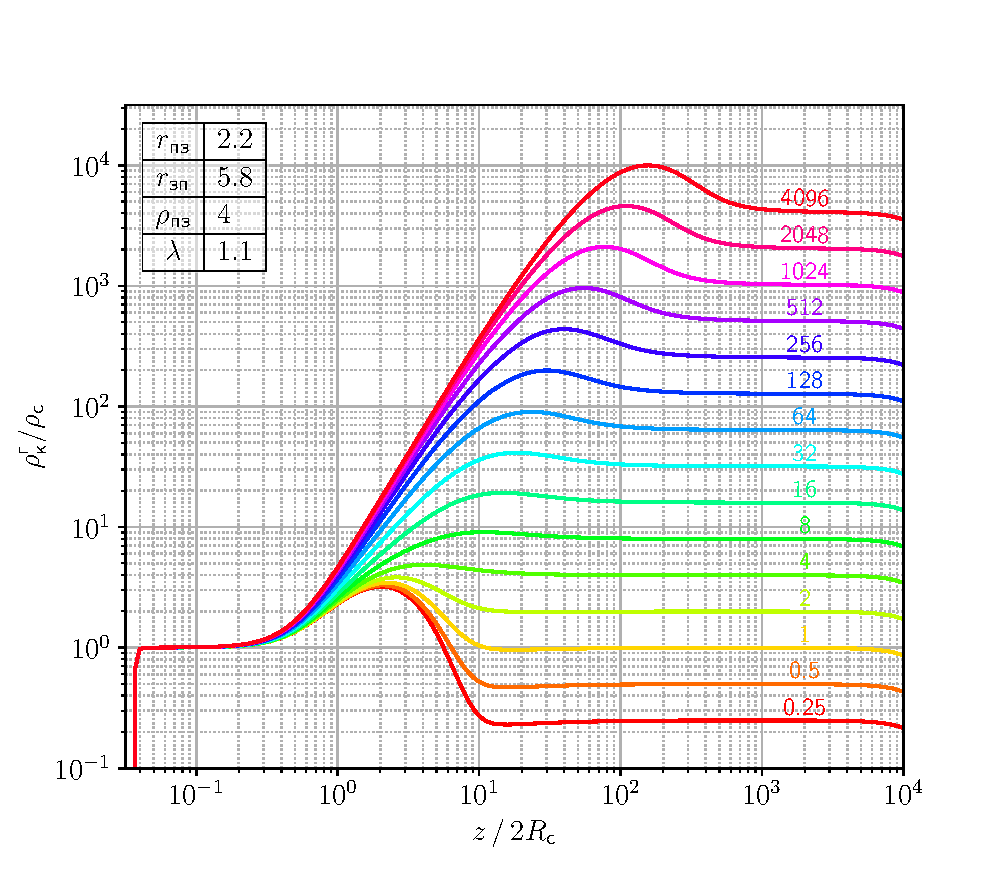
\includegraphics{plot_2_palette}
\caption{}
\end{figure}

Время вычисления палетки $16.5 \text{ c } \pm 176 \text{ мс}$, 7 проходов.

\clearpage
